\documentclass{article}
\usepackage[utf8]{inputenc}
\usepackage{amsmath, amssymb, tikz, geometry, multicol}
\usepackage{pgfplots}
\pgfplotsset{compat=1.17}
\geometry{margin=0.5in}
\setlength{\columnsep}{1cm}
\usepackage{siunitx}
\usepackage{booktabs}
\usepackage{hyperref}

\begin{document}

\begin{multicols}{2}

\section*{Time Dilation in Special Relativity}

\subsection*{Lorentz Factor}

The Lorentz factor (\(\gamma\)) describes how time dilates for an object moving at velocity \(v\) relative to an observer:

\[
\gamma = \frac{1}{\sqrt{1 - \left( \dfrac{v}{c} \right)^2 }}
\]

where:
- \( v \) = velocity of the moving object,
- \( c \) = speed of light (\( c = 299,792,458\, \text{m/s} \)).

\subsection*{Time Dilation Formula}

The relationship between time intervals measured in different frames:

\[
\Delta t = \gamma \Delta t'
\]

- \( \Delta t' \) = time interval measured in the \textbf{moving frame} (proper time),
- \( \Delta t \) = time interval measured in the \textbf{stationary frame}.

\subsection*{Time Difference}

The time difference (\( \Delta \tau \)) between the two frames:

\[
\Delta \tau = \Delta t - \Delta t' = \Delta t' (\gamma - 1)
\]

\subsection*{Calculations}

We will calculate the Lorentz factor and time difference for velocities ranging from \( 0 \) to \( c \).

\subsubsection*{Example Velocities}

Let’s consider the following velocities:

\[
v = 0.1c,\ 0.5c,\ 0.9c,\ 0.99c,\ 0.999c
\]

\subsubsection*{Calculations for Each Velocity}

\textbf{1. Calculate \( \gamma \):}

\[
\gamma = \frac{1}{\sqrt{1 - \left( \dfrac{v}{c} \right)^2 }}
\]

\textbf{2. Assume \( \Delta t' = 1\, \text{s} \), calculate \( \Delta t \) and \( \Delta \tau \):}

\[
\Delta t = \gamma \Delta t'
\]
\[
\Delta \tau = \Delta t - \Delta t' = (\gamma - 1) \Delta t'
\]

\subsubsection*{Tabulated Results}

\begin{center}
\begin{tabular}{@{}ccccc@{}}
\toprule
\( v \) & \( v/c \) & \( \gamma \) & \( \Delta t \) (s) & \( \Delta \tau \) (s) \\
\midrule
\( 0.1c \) & 0.1 & 1.0050 & 1.0050 & 0.0050 \\
\( 0.5c \) & 0.5 & 1.1547 & 1.1547 & 0.1547 \\
\( 0.9c \) & 0.9 & 2.2942 & 2.2942 & 1.2942 \\
\( 0.99c \) & 0.99 & 7.0888 & 7.0888 & 6.0888 \\
\( 0.999c \) & 0.999 & 22.3663 & 22.3663 & 21.3663 \\
\bottomrule
\end{tabular}
\end{center}

\subsection*{Plots of Lorentz Factor and Time Difference}

\subsubsection*{Plot of \( v \) vs. \( \gamma \)}

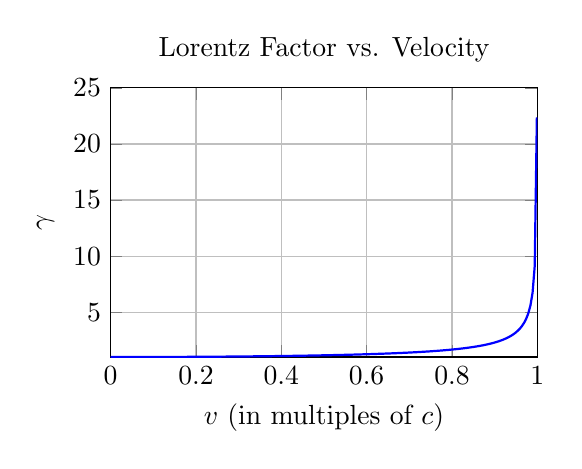
\begin{tikzpicture}
\begin{axis}[
    width=7cm,
    height=5cm,
    xlabel={$v$ (in multiples of $c$)},
    ylabel={\( \gamma \)},
    xmin=0, xmax=1,
    ymin=1, ymax=25,
    grid=both,
    title={Lorentz Factor vs. Velocity},
    ytick={0,5,10,15,20,25},
    legend style={at={(0.5,-0.2)},anchor=north}
]
\addplot [domain=0:0.999, samples=200, thick, blue] {1 / sqrt(1 - x^2)};
\end{axis}
\end{tikzpicture}

\subsubsection*{Plot of \( v \) vs. \( \Delta \tau \)}

Assuming \( \Delta t' = 1\, \text{s} \).

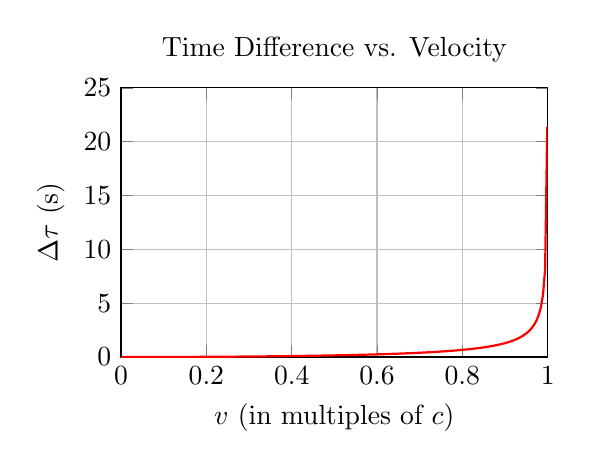
\begin{tikzpicture}
\begin{axis}[
    width=7cm,
    height=5cm,
    xlabel={$v$ (in multiples of $c$)},
    ylabel={\( \Delta \tau \) (s)},
    xmin=0, xmax=1,
    ymin=0, ymax=25,
    grid=both,
    title={Time Difference vs. Velocity},
    ytick={0,5,10,15,20,25},
    legend style={at={(0.5,-0.2)},anchor=north}
]
\addplot [domain=0:0.999, samples=200, thick, red] {(1 / sqrt(1 - x^2) - 1)};
\end{axis}
\end{tikzpicture}

\columnbreak

\section*{Energy Requirements}

\subsection*{Relativistic Kinetic Energy}

The kinetic energy (\( KE \)) required to accelerate an object to a relativistic speed is:

\[
KE = (\gamma - 1) m c^2
\]

where:
- \( m \) = rest mass of the object,
- \( \gamma \) = Lorentz factor,
- \( c \) = speed of light.

\subsection*{Calculations for the DeLorean}

Assuming the DeLorean has a mass \( m = 1,230\, \text{kg} \).

\subsubsection*{Calculations at Various Speeds}

\begin{enumerate}
    \item \( v = 0.1c \): \( \gamma = 1.0050 \)
    \item \( v = 0.5c \): \( \gamma = 1.1547 \)
    \item \( v = 0.9c \): \( \gamma = 2.2942 \)
    \item \( v = 0.99c \): \( \gamma = 7.0888 \)
    \item \( v = 0.999c \): \( \gamma = 22.3663 \)
\end{enumerate}

\textbf{Calculate \( KE \) for each velocity:}

\[
KE = (\gamma - 1) m c^2
\]

\subsubsection*{Tabulated Results}

\begin{center}
\begin{tabular}{@{}cccc@{}}
\toprule
\( v \) & \( \gamma \) & \( KE \) (J) & \( KE \) (\( 10^{16} \) J) \\
\midrule
\( 0.1c \) & 1.0050 & \( 3.328 \times 10^{16} \) & 0.3328 \\
\( 0.5c \) & 1.1547 & \( 1.066 \times 10^{18} \) & 10.66 \\
\( 0.9c \) & 2.2942 & \( 2.205 \times 10^{19} \) & 220.5 \\
\( 0.99c \) & 7.0888 & \( 6.583 \times 10^{19} \) & 658.3 \\
\( 0.999c \) & 22.3663 & \( 2.078 \times 10^{20} \) & 2078 \\
\bottomrule
\end{tabular}
\end{center}

\subsection*{Plot of \( v \) vs. \( KE \)}

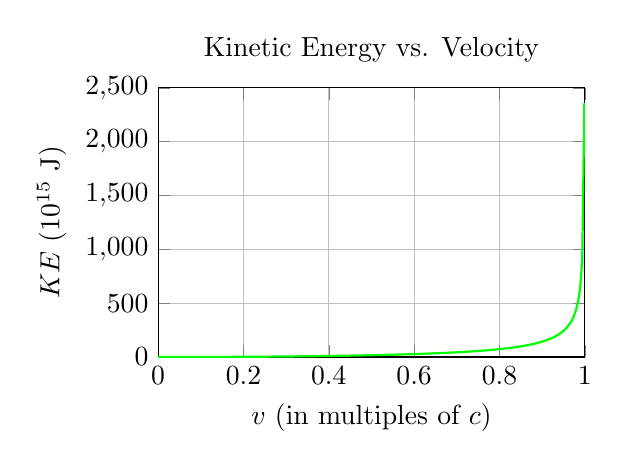
\begin{tikzpicture}
\begin{axis}[
    width=7cm,
    height=5cm,
    xlabel={$v$ (in multiples of $c$)},
    ylabel={$KE$ (\( 10^{15} \) J)},
    xmin=0, xmax=1,
    ymin=0, ymax=2500,
    grid=both,
    title={Kinetic Energy vs. Velocity},
    ytick={0,500,1000,1500,2000,2500},
    legend style={at={(0.5,-0.2)},anchor=north}
]
\addplot [domain=0:0.999, samples=200, thick, green] {(1 / sqrt(1 - x^2) - 1) * 1.230 * (2.99792458e8)^2 / 1e15};
\end{axis}
\end{tikzpicture}

\subsection*{Energy from Hydrogen Fusion}

\textbf{Energy Released per Fusion Reaction:}

In the proton-proton chain reaction (dominant in stars like the Sun), four protons fuse to form a helium nucleus, releasing about \( 26.7\, \text{MeV} \) per reaction.

\[
E_{\text{fusion}} = 26.7\, \text{MeV} = 4.28 \times 10^{-12}\, \text{J}
\]

\textbf{Energy per Kilogram of Hydrogen:}

Mass of four protons:

\[
m_{\text{protons}} = 4 \times 1.6726 \times 10^{-27}\, \text{kg} = 6.6904 \times 10^{-27}\, \text{kg}
\]

Number of reactions per kg of hydrogen:

\[
N = \frac{1\, \text{kg}}{6.6904 \times 10^{-27}\, \text{kg}} \approx 1.495 \times 10^{26}
\]

Total energy per kg of hydrogen:

\[
E_{\text{total}} = N \times E_{\text{fusion}} = (1.495 \times 10^{26}) \times (4.28 \times 10^{-12}\, \text{J}) \approx 6.4 \times 10^{14}\, \text{J}
\]

\subsection*{Calculating Mass of Hydrogen Needed}

\textbf{For \( v = 0.9c \):}

Energy required:

\[
KE = 2.205 \times 10^{19}\, \text{J}
\]

Mass of hydrogen needed:

\[
m_{\text{H}} = \frac{KE}{E_{\text{total per kg}}} = \frac{2.205 \times 10^{19}\, \text{J}}{6.4 \times 10^{14}\, \text{J/kg}} \approx 34,453\, \text{kg}
\]

\textbf{For \( v = 0.99c \):}

Energy required:

\[
KE = 6.583 \times 10^{19}\, \text{J}
\]

Mass of hydrogen needed:

\[
m_{\text{H}} = \frac{6.583 \times 10^{19}\, \text{J}}{6.4 \times 10^{14}\, \text{J/kg}} \approx 102,859\, \text{kg}
\]

\textbf{For \( v = 0.999c \):}

Energy required:

\[
KE = 2.078 \times 10^{20}\, \text{J}
\]

Mass of hydrogen needed:

\[
m_{\text{H}} = \frac{2.078 \times 10^{20}\, \text{J}}{6.4 \times 10^{14}\, \text{J/kg}} \approx 324,688\, \text{kg}
\]

\subsubsection*{Summary Table}

\begin{center}
\begin{tabular}{@{}cccc@{}}
\toprule
\( v \) & \( KE \) (\( 10^{19} \) J) & \( m_{\text{H}} \) (kg) & \( m_{\text{H}} \) (tonnes) \\
\midrule
\( 0.9c \) & 2.205 & 34,453 & 34.5 \\
\( 0.99c \) & 6.583 & 102,859 & 102.9 \\
\( 0.999c \) & 20.78 & 324,688 & 324.7 \\
\bottomrule
\end{tabular}
\end{center}

\subsection*{Interpretation}

- Accelerating the DeLorean to relativistic speeds requires immense amounts of energy.
- Even with efficient hydrogen fusion, large masses of hydrogen would be needed.
- For \( v = 0.999c \), over 324 tonnes of hydrogen would be required.

\section*{Key Equations Summary}

\subsection*{Lorentz Factor}

\[
\gamma = \frac{1}{\sqrt{1 - \left( \dfrac{v}{c} \right)^2 }}
\]

\subsection*{Time Dilation}

\[
\Delta t = \gamma \Delta t'
\]

\subsection*{Time Difference}

\[
\Delta \tau = \Delta t - \Delta t' = \Delta t' (\gamma - 1)
\]

\subsection*{Relativistic Kinetic Energy}

\[
KE = (\gamma - 1) m c^2
\]

\subsection*{Energy from Fusion}

\[
E_{\text{fusion per kg}} \approx 6.4 \times 10^{14}\, \text{J/kg}
\]

\end{multicols}

\end{document}
